% --- Program Section ---

\newprogram{Program 10}{Implement longestCommonSubsequence(text1: str, text2: str) -> int and
minDistance(word1: str, word2: str) -> int functions accepting input strings and returning
optimal length/edit operation counts.}

\subsection*{Code}


\begin{lstlisting}[language=python]
def longestCommonSubsequence(text1: str, text2: str) -> int:
    m = len(text1)
    n = len(text2)

    dp = [[0] * (n + 1) for _ in range(m + 1)]

    for i in range(1, m + 1):
        for j in range(1, n + 1):

            if text1[i - 1] == text2[j - 1]:
                dp[i][j] = 1 + dp[i - 1][j - 1]
            else:
                dp[i][j] = max(dp[i - 1][j], dp[i][j - 1])

    return dp[m][n]


def minDistance(word1: str, word2: str) -> int:
    m = len(word1)
    n = len(word2)

    dp = [[0] * (n + 1) for _ in range(m + 1)]

    # Converting empty string to word2
    for j in range(n + 1):
        dp[0][j] = j

    # Converting word1 to empty string
    for i in range(m + 1):
        dp[i][0] = i

    for i in range(1, m + 1):
        for j in range(1, n + 1):

            if word1[i - 1] == word2[j - 1]:
                dp[i][j] = dp[i - 1][j - 1]
            else:
                dp[i][j] = 1 + min(
                    dp[i - 1][j],      # Delete
                    dp[i][j - 1],      # Insert
                    dp[i - 1][j - 1]   # Replace
                )

    return dp[m][n]


# Examples

print(longestCommonSubsequence("abcde", "ace"))
print(minDistance("horse", "ros"))
\end{lstlisting}

\subsection*{Output}
\begin{center}
    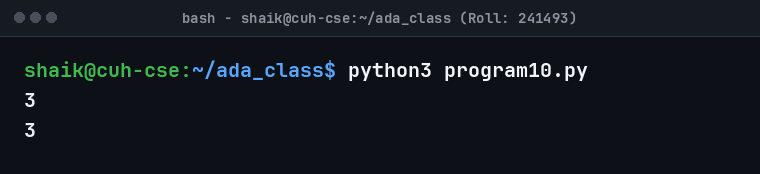
\includegraphics[width=0.88\textwidth]{Images/output_screenshot10.png}
\end{center}

\subsection*{GitHub Scan Code}
\begin{center}
    \begin{minipage}{0.3\textwidth}
        \centering
        % Generates a 2.5cm high QR code directly linking to the code file
        \qrcode[height=3.5cm]{https://github.com/gytdrop/ada_class/blob/main/program10.py} \\[0.2cm]
        \scriptsize\ttfamily Scan to view source code 
    \end{minipage}
\end{center}


% Add a horizontal line that indicates the END of the program.
\vspace{1cm}
\begin{center}
    \rule{1\textwidth}{1pt} % Clean, centered 1pt thick horizontal line
\end{center}